\section{Transcriptions using Transkribus}



%-----------------------------------------------------
\begin{frame}[allowframebreaks,fragile]{Transcription}
\subsubsection{Transcription}
\metroset{block=fill}

\begin{columns}
\column{0.48\textwidth}
\begin{itemize}\small
\item  OCR (Optical Character Recognition) -- e.g. Transkribus (transcription support)
\item  Transkribus Keyword Spotting 
\item  fuzzy search which should also find the word if it's mistranscribed
\item  Writer identification
\end{itemize}

\column{0.48\textwidth}

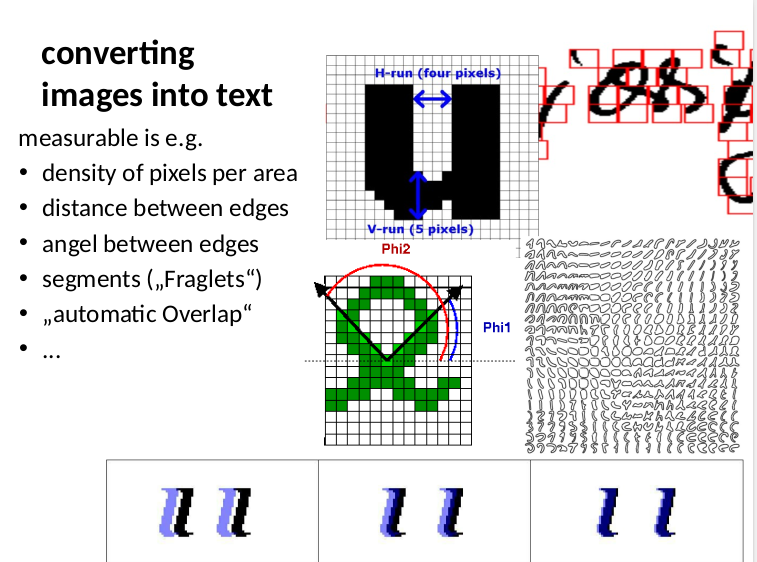
\includegraphics[width=\textwidth]{img/ocr1.png}
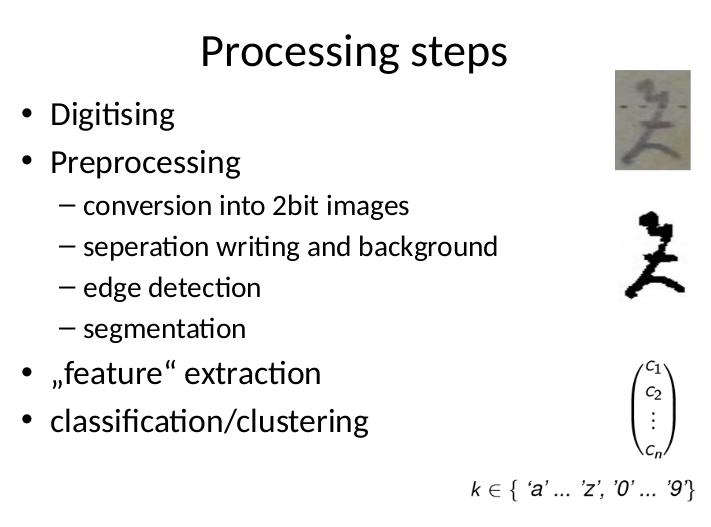
\includegraphics[width=\textwidth]{img/ocr2.png}
\end{columns}

\framebreak 

\begin{columns}
\column{0.48\textwidth}
\begin{block}{Typical phenomena}
\begin{itemize}
\item “Special characters"
\item Abbreviations
\item damaged or unreadable text
\item additions, deletions, substitutions, corrections
\item editorial interventions (emendations and conjectures)
\item  editorial additions or omissions
\end{itemize}
\end{block}

\column{0.48\textwidth}

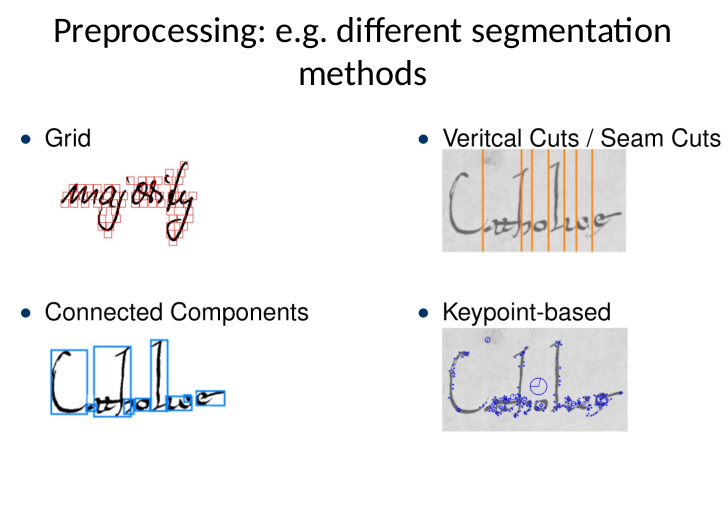
\includegraphics[width=\textwidth]{img/ocr3.png}
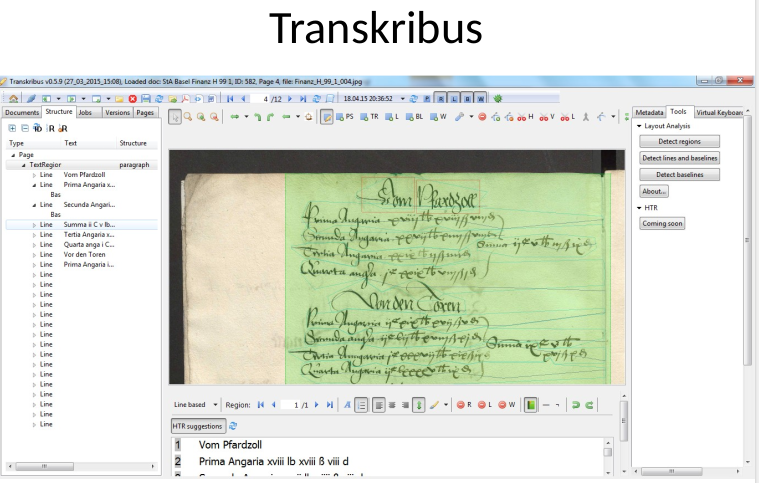
\includegraphics[width=\textwidth]{img/ocr4-transkribus-app.png}

\end{columns}

\end{frame}
%-----------------------------------------------------

\begin{frame}{What is Transkribus?}
    \begin{block}{Transkribus}
       \begin{quote}
           \dots{}is a comprehensive platform for the digitisation, AI-powered text recognition, transcription and searching of historical documents. (\href{https://readcoop.eu/transkribus/}{source})
       \end{quote}
    \end{block}
    \begin{itemize}
        \item we're using the web version TranskribusLite: \protect\url{https://transkribus.eu/lite}
        \begin{itemize}
            \item for more complexity (which you might not need), download the software (Transkribus eXpert)
            \item Lite is easier to learn \& has only the essentials.
            \item you need an account and to buy credits after you have used up your initial 200
            \item print \& manuscript text recognition have different pricing
            \item there are stipends
        \end{itemize}        
    \end{itemize}
\end{frame}


%-----------------------------------------------------
\begin{frame}{Transkribus: Lite versus eXpert}
    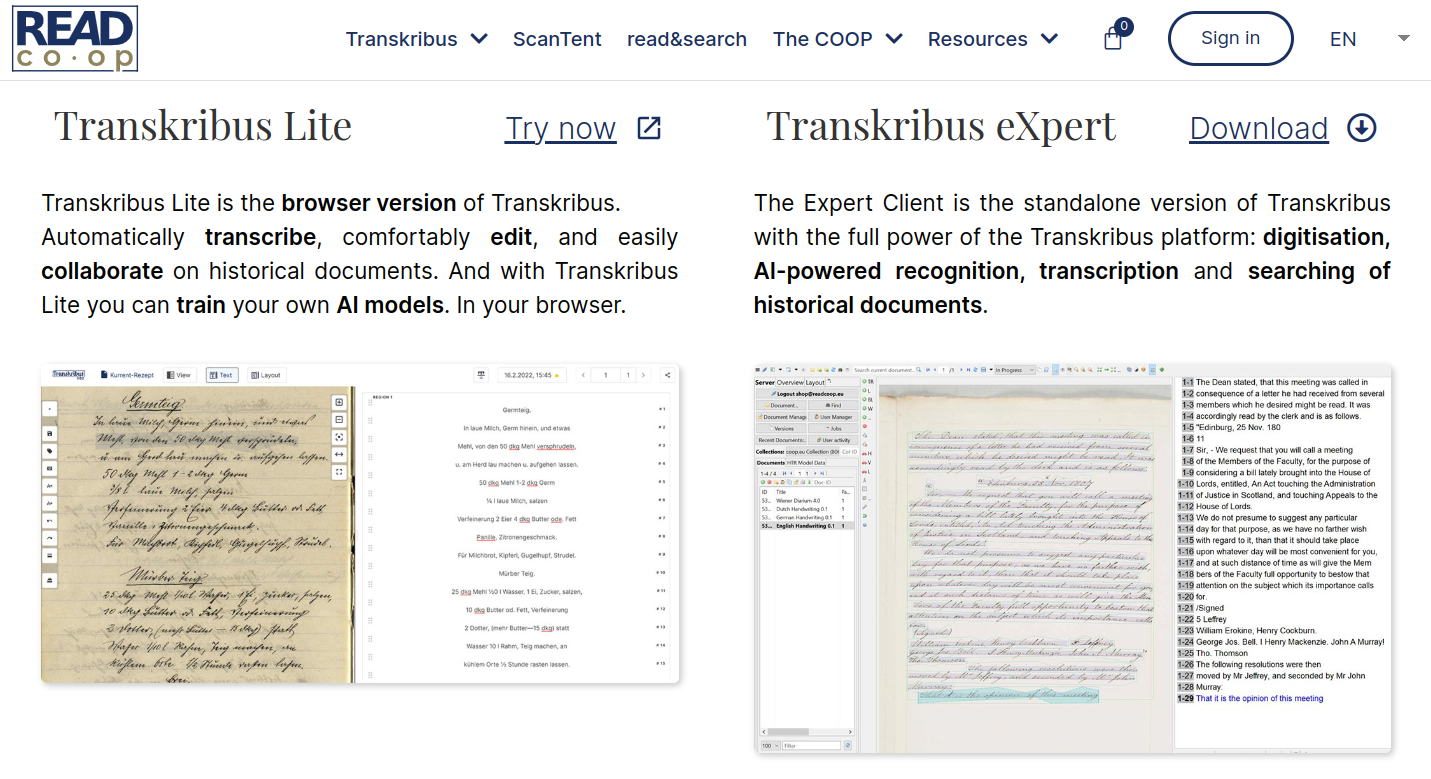
\includegraphics[width=0.95\textwidth]{img/transkribus-versions.png}
\end{frame}
%-----------------------------------------------------
\begin{frame}{Transkribus: How to guides}
    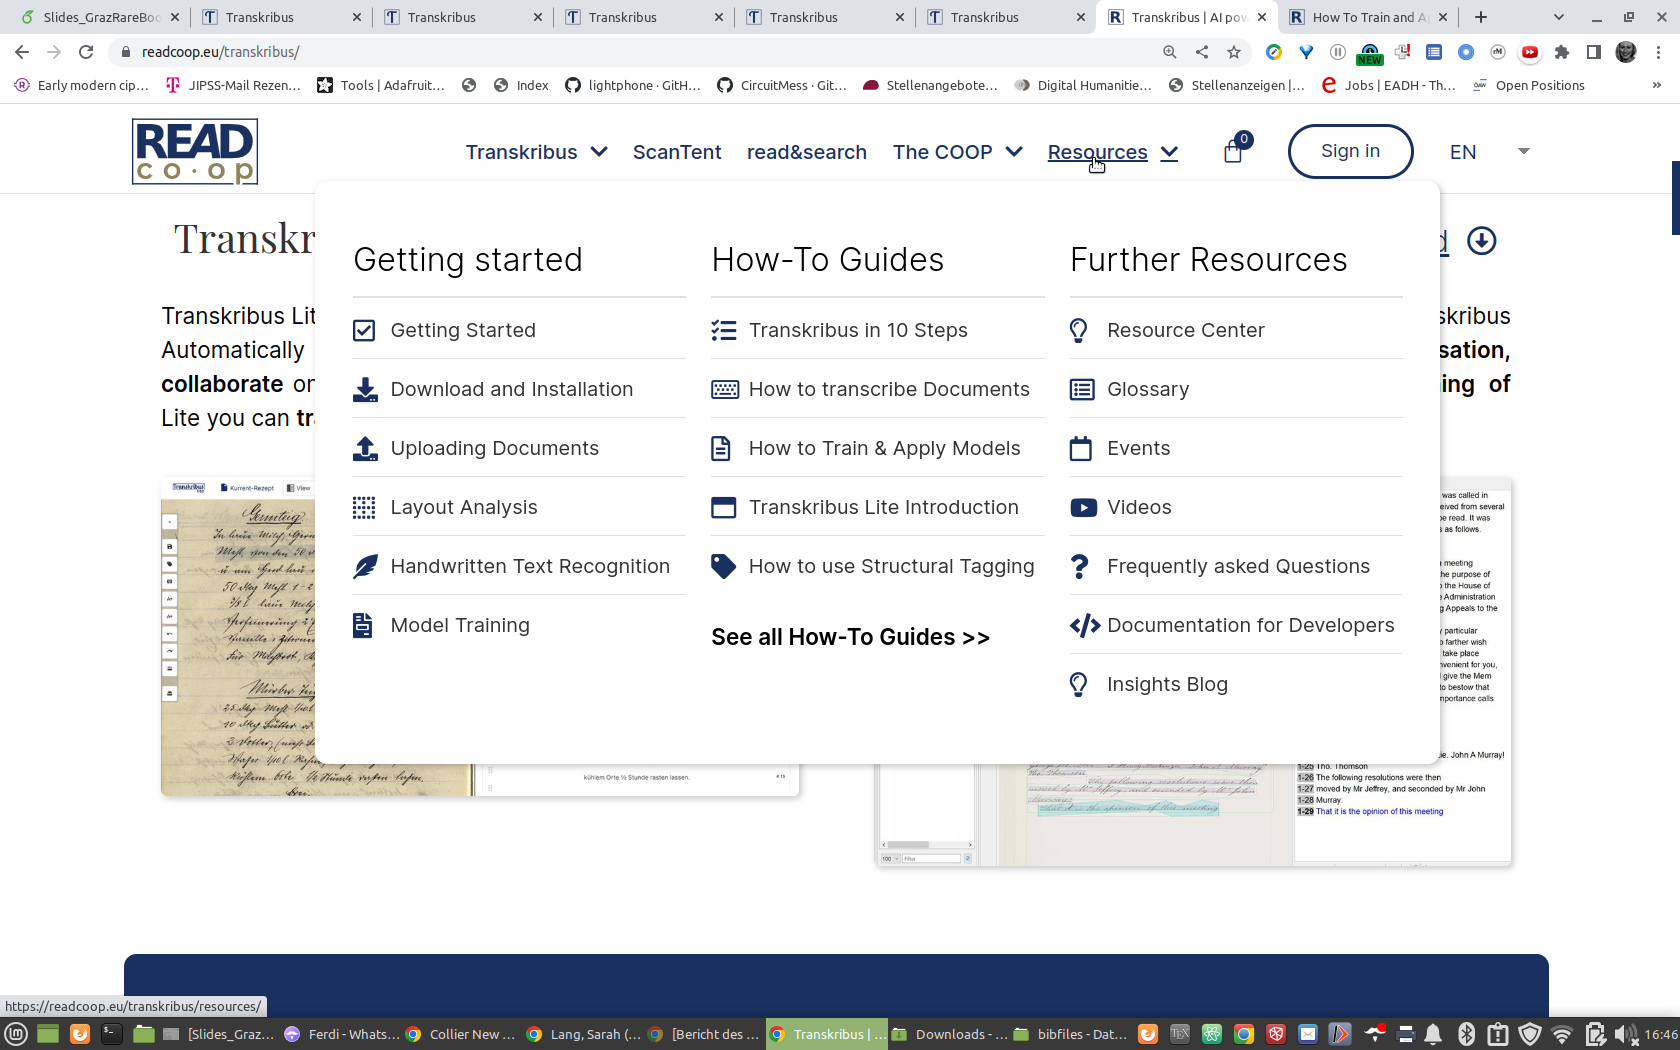
\includegraphics[width=0.95\textwidth]{img/transkribus-resources.png}
\end{frame}
%-----------------------------------------------------
\begin{frame}{Transkribus: Creating transcriptions to train your own model}
    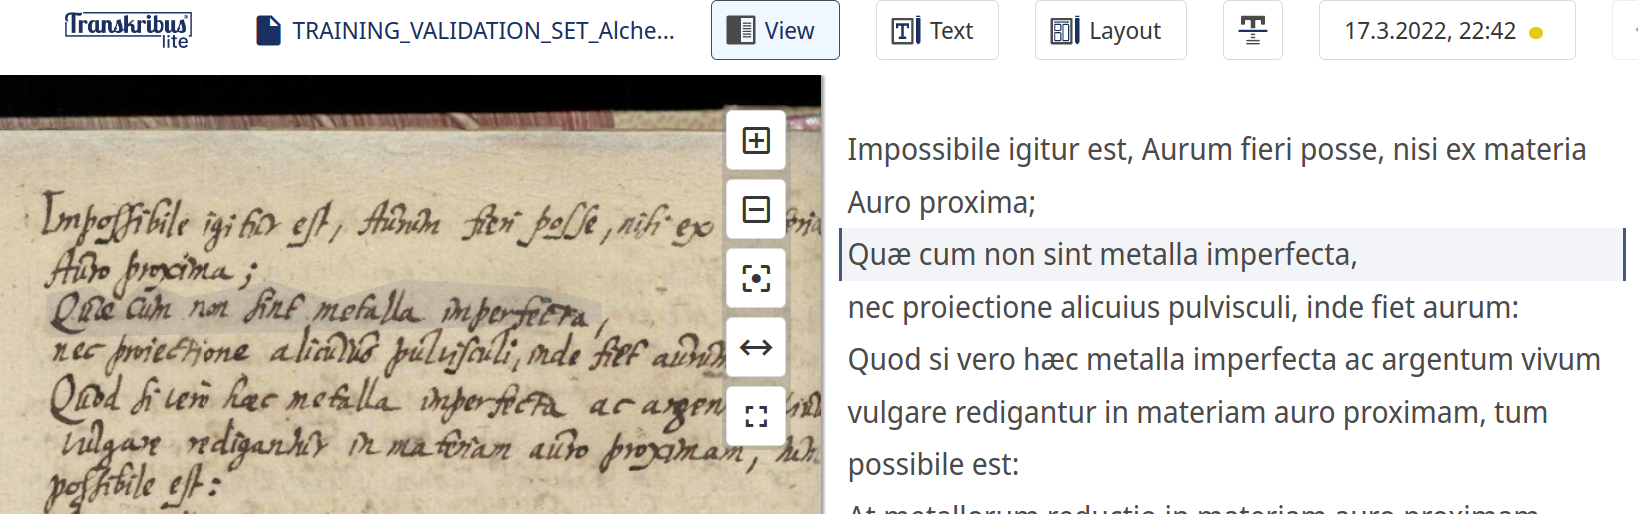
\includegraphics[width=0.95\textwidth]{img/transkribus-training1.png}
    \begin{itemize}\small
        \item first, transcribe a number of pages 
        \begin{itemize}\footnotesize
            \item recommended: 25--75
            \item depending on print or handwritten
            \item you can build on base models (should be similar)
            \item you can speed up the process by creating a model, running it on new pages, correcting them and then repeating the process
            \item correcting is usually still faster than transcribing from scratch
        \end{itemize}
        \item be mindful to adhere to the transcription guidelines you want the model to learn
        \item train your model using the gold-standard transcriptions
        \item use the model on the pages you want transcribed
        \item there will probably be errors: fix them \& use the extra training data created thus to improve the model by retraining it
        \item consider publishing your model if it's of reusable quality
    \end{itemize}
\end{frame}
%-----------------------------------------------------
\begin{frame}{Transkribus: Configuring your model}
    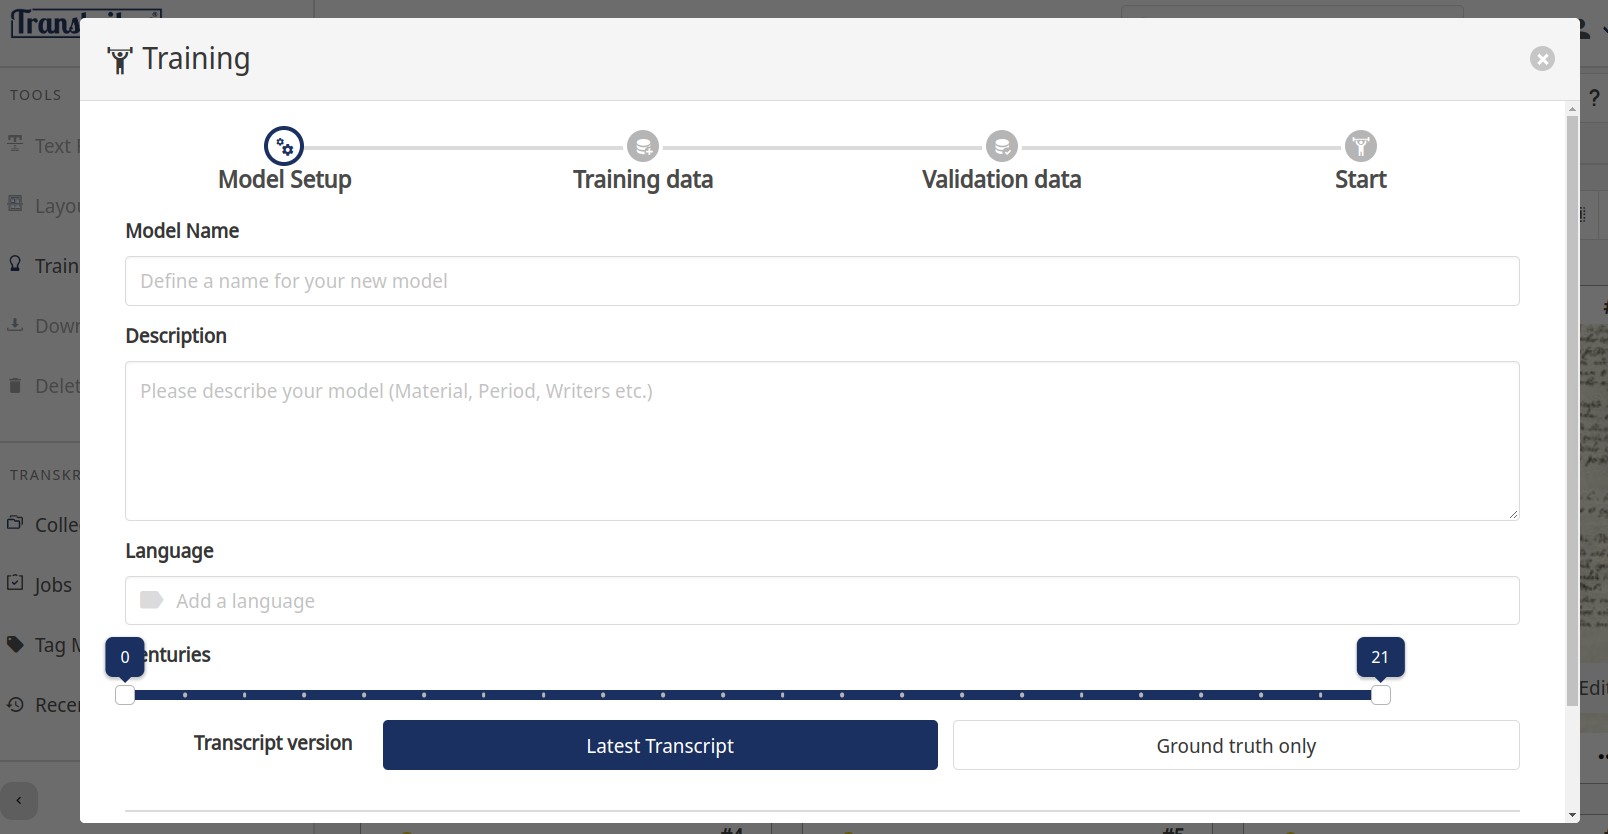
\includegraphics[width=0.95\textwidth]{img/transkribus-training2.png}
\end{frame}


%-----------------------------------------------------
\begin{frame}{Transkribus: further resources}
    \begin{itemize}
        \item \emph{How to historical text recognition: A Transkribus Quickstart Guide}, \LaTeX{}-Ninja Blog, 10. November 2019, \href{https://latex-ninja.com/2019/11/10/how-to-historical-text-recognition-a-transkribus-quickstart-guide/}{URL}. \alert{$\to$ how to reuse exisiting models for print on the example of the Noscemus GM4}
        \item \emph{Training my own Handwritten Text Recognition (HTR) model on Transkribus Lite}, \LaTeX{}-Ninja Blog, 22. March 2022, \href{https://latex-ninja.com/2022/03/22/training-my-own-handwritten-text-recognition-htr-model-on-transkribus-lite/}{URL}. \alert{$\to$ experiences training my own model}
    \end{itemize}
\end{frame}

